\chapter{Crossline Deblending (3D)} \label{chap:MahdadMethod3d}

This thesis proposes to blend crossline sources. It is hypothesized that by combining several cross-lines one can effectively blend sources in 3D. Figure \ref{fig:Ch-Mahdad3d-Geometry_v2} illustrates how a 3D source grid can be built. Note that for 3D blending each cross-line must be fired with a different blending pattern. Otherwise the blending noise along the inline direction would be coherent.

\begin{figure}
	\centering
	\includegraphics[width = \textwidth]{Plots/AcquisitionDesign/Geometry_v3}	
	\caption{\textit{Top}: Illustration of the 3D source grid array. \textit{Bottom}: The vessels show how the source grid can be built in practice.}
	\label{fig:Ch-Mahdad3d-Geometry_v2}	
\end{figure}

The deblending method of \citet{Mahdad-Deblending-Method} described in section \ref{sec:MahdadMethod} is a 2D method. In this chapter I will derive a 3D deblending method, which is based on the Mahdad method, and I will demonstrate its strengths and  performance.

First, I will modify the data sorting such that the blended 3D data can be described using the same forward model as in section \ref{sec:Ch-Theory-Operator}. The presented data sorting will allow to maintain all other steps of the deblending algorithm of \citet{Mahdad-Deblending-Method}. Second, I will extend the incoherency estimation of the blending design from 2D to 3D. Third, I will extend the 2D $f$-$k$ filter to a 3D $f$-$k_x$-$k_y$ filter to attenuate blending noise in both crossline and inline direction.

\section{Data Sorting} \label{sec:Ch-Theory-3dExtension-DataSorting}

\subsection*{Data Matrix}

In 3D acquisition the sources and receivers are distributed on a 2D surface. Thus, their locations are defined by their inline and crossline positions, ($x$, $y$). Each data point which is measured by a source receiver pair at a specific time is therefore described by 5 coordinates, time $t$, receiver inline and crossline position ($x_r$, $y_r$), and source inline and crossline position ($x_s$, $y_s$).

Similar as in section \ref{sec:Ch-Theory-Operator} the 5D data "cube" will be again reorganized in a 2D data matrix according to \citet{Delphi-Format} (see Figure \ref{fig:Ch-Theory-DelphiFormat}). For this data sorting a 1D Fourier transform with respect to time is performed and a 4D frequency "slice" is selected.

The 4D "slice" is sorted in a 2D data matrix, $\mathbf{P}$, with as many rows as receivers and as many columns as shots. The total number of shots is obtained by multiplying the number of shots fired in each crossline and the number of shots fired in each inline. The total number of receivers is obtained likewise. Assume there are $Ns_x$ shots per crossline. The shots of the first crossline are assigned to the first $Ns_x$ columns of the data matrix, the shots of the second crossline are assigned to the next $Ns_x$ columns of the data matrix, etc. The receivers are sorted in the rows of the data matrix analogously.

\nomenclature{$Ns_x$}{Number of sources in crossline direction}
\nomenclature{$Ns_y$}{Number of sources in inline direction}
\nomenclature{$x$}{Crossline space coordinate}
\nomenclature{$y$}{Inline space coordinate}
\nomenclature{CRG}{Common-receiver gather}
\nomenclature{CSG}{Common-shot gather}

One row in the data matrix, $\mathbf{P}$, in Figure \ref{fig:Ch-Theory-DelphiFormat} represents  a 3D common-receiver gather. The data of this 3D common-receiver gather are shown in Figure \ref{fig:Ch-Theory-Data3d} in a 3D-view, where the coordinates, $x$ and $y$, indicate the inline and crossline shot position respectively. For the described data sorting individual crossline slices are extracted from this data cube and assembled next to each other in a data matrix as shown in Figure \ref{fig:Ch-Theory-Data3d_Delphi}. This view will be referred to as 3D-CRG 2D-view. Each hyperbolic event in Figure \ref{fig:Ch-Theory-DataSorting} refers to the response of the shots of one crossline.

\begin{figure}
	\centering
	\includegraphics[width=0.6\textwidth]{Plots/DelphiFormat-v3}
	\caption{Illustration of the data matrix $\mathbf{P}$ for 3D data \citep{Delphi-Format}. $y_r$ and $y_s$ represent the inline receiver and shot positions. $x_r$ and $x_s$ represent the crossline receiver and shot positions. Each row refers to a 3D common-receiver gather and each column to a 3D common-shot gather. A sub-matrix with fixed receiver and source inline positions ($y_r$, $y_s$) is equivalent to a data matrix for 2D acquisition.}
	\label{fig:Ch-Theory-DelphiFormat}
\end{figure}


\begin{figure}
	
	\begin{subfigure}[t]{\textwidth}
	 	\centering
		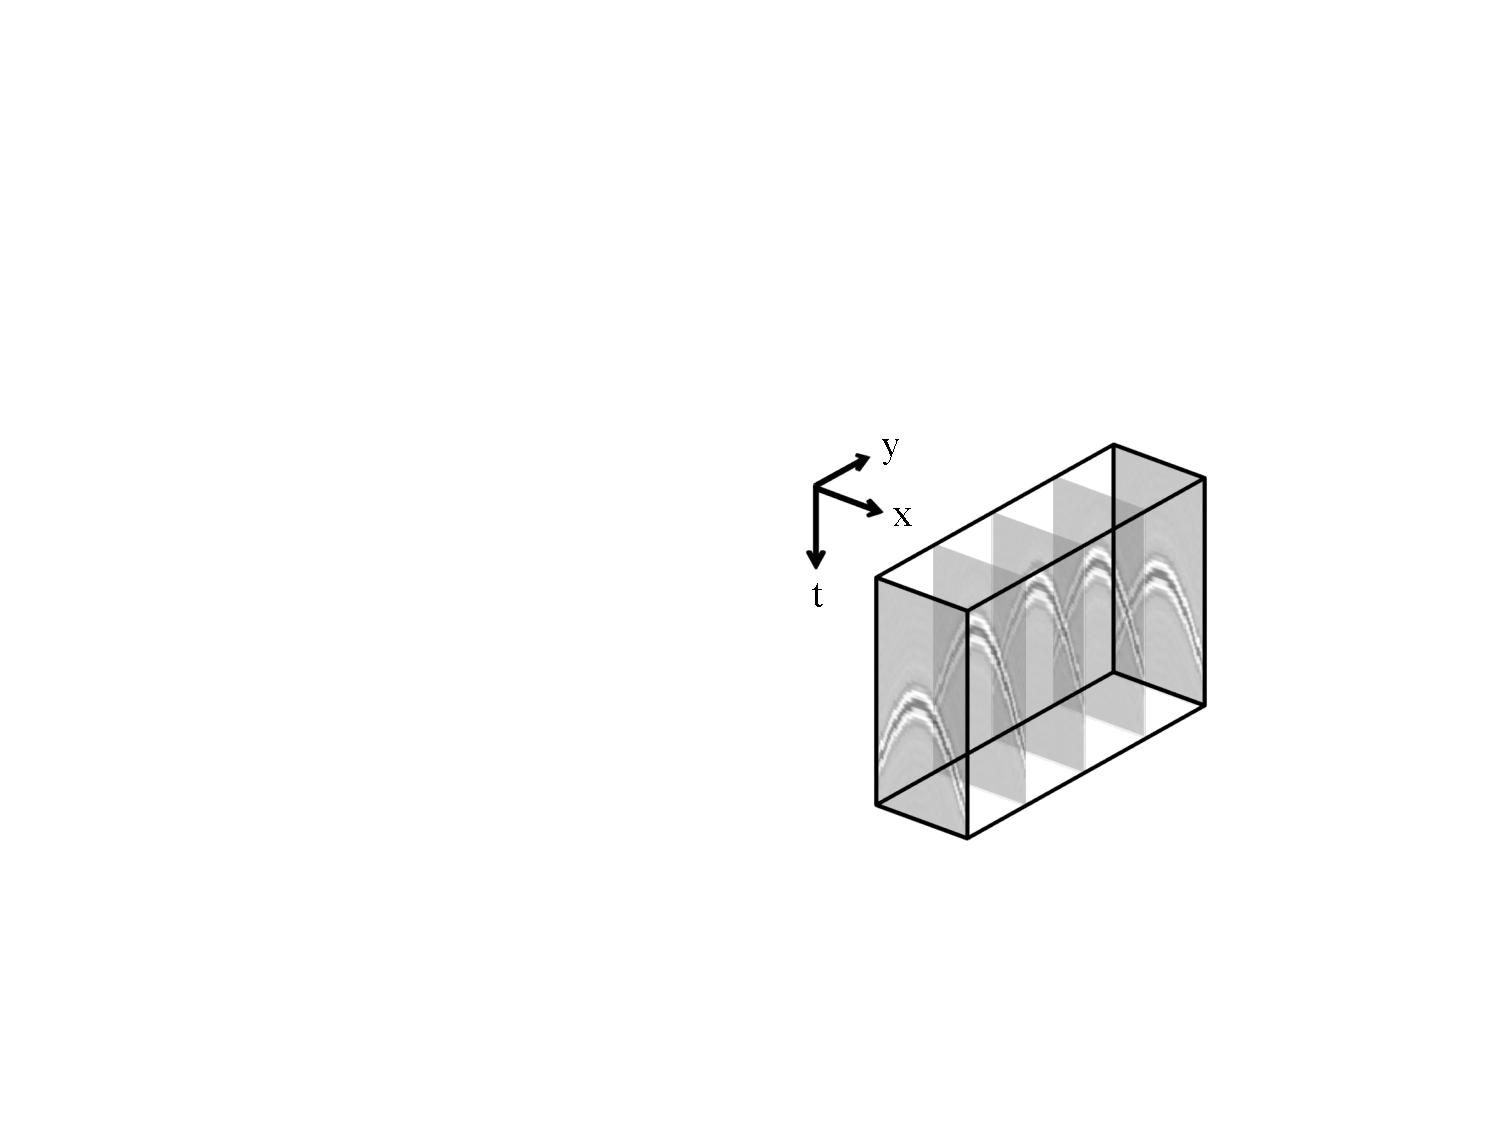
\includegraphics[width = 0.3\textwidth]{Plots/data3d}
		\caption{}
		\label{fig:Ch-Theory-Data3d}
	\end{subfigure}
	\par\bigskip
	\begin{subfigure}[t]{\textwidth}
		\centering
		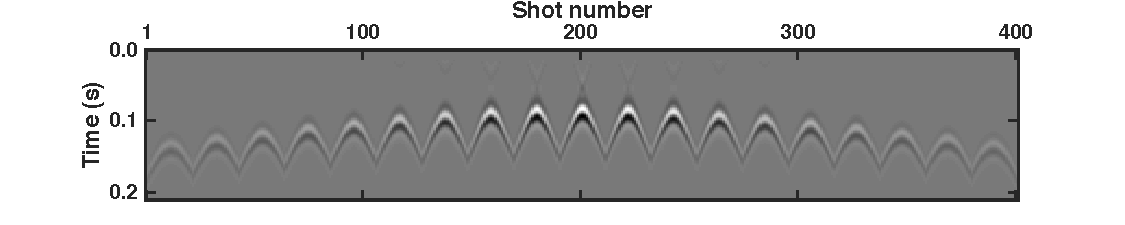
\includegraphics[width = \textwidth]{Plots/IdealData3d/p_Delphi}
		\caption{}
		\label{fig:Ch-Theory-Data3d_Delphi}
	\end{subfigure}
	
	\caption{(a) 3D common-receiver gather with crossline (x) and inline (y) sources (3D view). (b) Resorted data set. Individual crossline sections are plotted next to each other in 2D. For visibility both subfigures only show a reduced part of the data. This view is called 3D CRG 2D view.}
	\label{fig:Ch-Theory-DataSorting}
\end{figure}


\subsection*{Blending matrix}

The blending matrix for 3D is built in a similar fashion as the data matrix in 3D. As described in section \ref{sec:BlendingMatrix} each row of the blending matrix, $\mathbf{\Gamma}$, captures one shot. For extension to 3D the shots of the first crossline are placed in the top $Ns_x$ rows of the blending matrix, followed by the shots of the second crossline etc. (see Figure \ref{fig:Ch-Theory-3D-BlendingMatrix-Design}). The elements in the $j^{th}$ column of the blending matrix, $\mathbf{\Gamma}$, select the shots which are blended in the $j^{th}$ experiment. For example, the first column of the blending matrix in Figure \ref{fig:Ch-Theory-3D-BlendingMatrix} describes that in the first experiment shots (rows) $1$ and $3$ are blended with a time delay of $\Delta t_1$.

%\todo[inline]{Keep this sentence for later: This framework allows to blend any source combination independent of the cross- and inline positions of the involved sources.}

With the new data and blending matrix sorting one can apply deblending to 3D data in the same way as presented in section \ref{sec:Ch-Theory-Operator} and section \ref{sec:MahdadMethod}. Note that unlike for 2D blending spatially incoherent blending patterns are practical for blended crossline sources (3D).

\begin{figure}

	\begin{subfigure}[t]{0.5\textwidth}
		\centering
		\includegraphics[width = \textwidth]{Plots/DrawingsCartesianFormat4}
		\caption{}
		\label{fig:Ch-Theory-3D-BlendedAcquisition}
	\end{subfigure}
	%
	\begin{subfigure}[t]{0.5\textwidth}
		\centering
		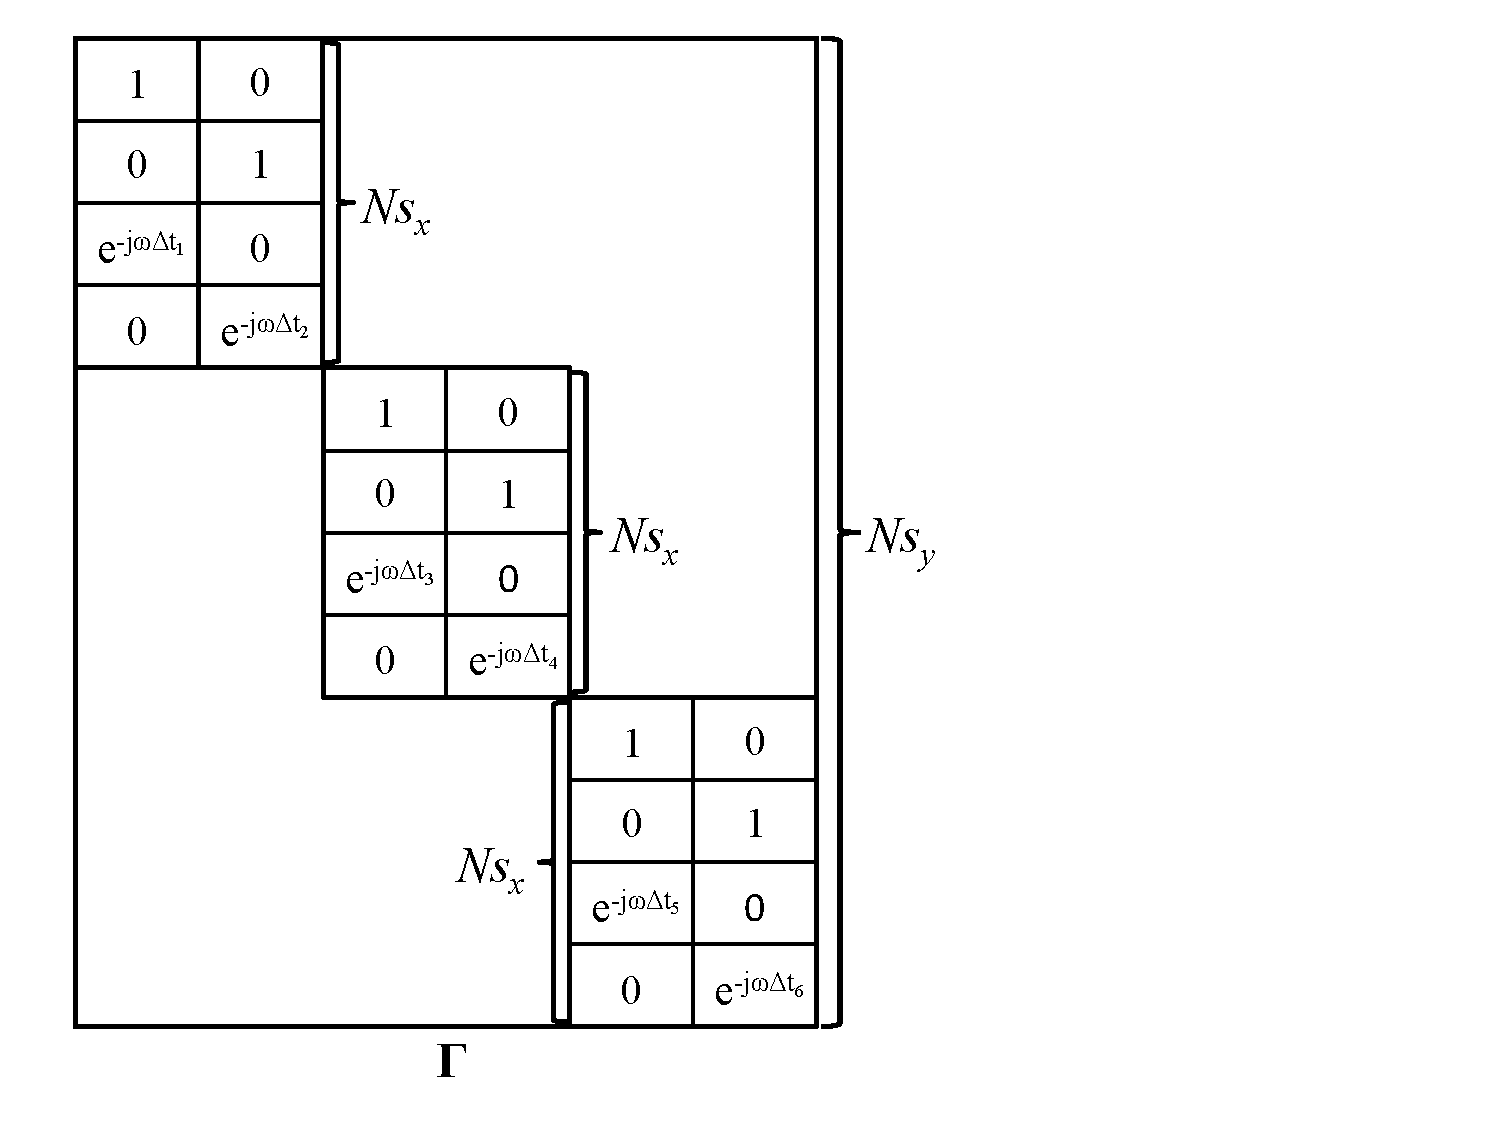
\includegraphics[width = 0.7\textwidth]{Plots/DrawingsCartesianFormat2}
		\caption{}
		\label{fig:Ch-Theory-3D-BlendingMatrix}
	\end{subfigure}
	
	\caption{Illustration of the blending matrix, $\mathbf{\Gamma}$, for 3D acquisition. (a) At each of the $Ns_y$ inline position the crossline sources ($x$ direction) are blended. Each of these 2D blending processes is described by a 2D blending matrix, which has as many rows as there are crossline sources, $Ns_x$. (b) The 2D blending matrices are assembled in a single 3D blending matrix, $\mathbf{\Gamma}$, which has $Ns_x$ by $Ns_y$ rows.}
	\label{fig:Ch-Theory-3D-BlendingMatrix-Design}

\end{figure}

\section{Incoherency}

The incoherency value is calculated in a similar way as in the 2D case (see chapter \ref{chap:Incoherency}). Due to the data sorting presented in section \ref{sec:Ch-Theory-3dExtension-DataSorting} the definition of the incoherency value requires some modifications.

Assume the blending matrix, $\mathbf{\Gamma}$, is sorted as described in section \ref{sec:Ch-Theory-3dExtension-DataSorting}. Hence, along the main diagonal of the matrix product, $\mathbf{\Gamma \Gamma}^H$, there are as many sub-matrices as there are inline sources, $Ns_y$. Each sub-matrix has as many rows and columns as there are crossline sources, $Ns_x$.

Each sub-matrix can be considered as a "small version" of the matrix product, $\mathbf{\Gamma \Gamma}^H$, which refers to a single cross-line. A 2D incoherency value is computed for each of these sub-matrices (see chapter \ref{chap:Incoherency}). The mean of these incoherency values is defined as the 3D incoherency value, $\mu$. Note that this definition captures the incoherency along the crossline direction. As in this thesis sources are not blended along the inline direction, the incoherency along the inline direction equals one.

\begin{comment}
\subsection*{Inline Incoherency}

In order to determine the inline incoherency, $\mu_y$, the blending matrix, $\mathbf{\Gamma}$, must be re-sorted. The sorting is analogous to the sorting in Figure \ref{fig:Ch-Theory-3D-BlendingMatrix}, except that the crossline and inline sources are interchanged. Thus, the sources of the first inline are sorted in the first $Ns_y$ rows of the blending matrix. The sources of the second inline are sorted in the next $Ns_y$ rows of the blending matrix, etc.

Subsequently, the inline incoherency value is calculated analogously to the crossline incoherency value.
\end{comment}

\section{3D $f$-$k_x$-$k_y$ Filter} \label{sec:Ch-Theory-3dExtension-FKK}

In section \ref{sec:IterBlenNoiseEst} the 2D $f$-$k$ filter was introduced. In 3D there are two spatial directions ($x$,$y$), i.e. the filter can be extended to a 3D $f$-$k_x$-$k_y$ filter.

For this purpose one considers a 3D common-receiver gather, $\mathbf{p}(t,x_s,y_s)$, and brings it to the $f$-$k_x$-$k_y$ domain by applying a 3-dimensional Fourier transform. Next, a constant frequency slice is selected. This leaves a 2D matrix, which captures the crossline and inline wavenumbers ($k_x$, $k_y$) as shown in Figure \ref{fig:Ch-Theory-FK-f_slice-data}. Note that the data map in a circle.


The lowest wavefield velocity, $v_{min}$, and the frequency, $f$, determine the maximum wavenumber, $k_{max}$, according to equation \ref{eq_Ch-Theory-MaxWavenmber};

\begin{equation}
	k_{max} = \frac{f}{v_{min}}.
	\label{eq_Ch-Theory-MaxWavenmber-Repetition}
\end{equation} 

The total wavenumber, $k_{T}$, must be smaller than the maximum wavenumber, $k_{max}$,

\begin{equation}
	k_{T} = \sqrt{k_x^2 + k_{y}^2} < k_{max}.
	\label{eq:Ch-Theory-TotalWavenumber}
\end{equation}
\nomenclature{$k_T$}{Total wavenumber}

Hence the signal "cone" is defined by a circle in the $k_x$-$k_y$ domain (see Figure \ref{fig:Ch-Theory-FK-f_slice-mask}). This is repeated for each frequency component, such that the overall $f$-$k_x$-$k_y$ mask is a 3D cone (see Figure \ref{fig:Ch-Theory-FK-f_slice-data3d}). The cone can be sorted in a 2D view according to section \ref{sec:Ch-Theory-3dExtension-DataSorting} as illustrated in Figure \ref{fig:Ch-Theory-FK-delphi-data} and Figure \ref{fig:Ch-Theory-FK-delphi-mask}. 

For comparison, a 2D $f$-$k$ filter is designed for 3D data by copying the 2D $f$-$k$ filter along the inline direction. The resulting filter is  plotted in a 2D-view in Figure \ref{fig:Ch-Mahdad3d-2dfk}. Note that the 3D $f$-$k_x$-$k_y$ filter (see Figure \ref{fig:Ch-Theory-FKK-Mask}) removes significantly more incoherent energy than the 2D $f$-$k$ filter. 

%The maximum crossline wavenumber, $k_x$, is defined according to section \ref{sec:IterBlenNoiseEst}. The resulting $f$-$k$-mask is shown in Figure \ref{fig:Ch-Mahdad3d-2dfk}. Note that it only filters the crossline wavenumbers $k_x$, i.e. it is a $f$-$k_x$ filter.

%The $f$-$k_x$-$k_y$ spectra of synthetic data shown in Figure \ref{fig:Ch-Theory-FK-f_slice-data} and \ref{fig:Ch-Theory-FK-delphi-data} illustrate that the 2D $f$-$k_x$-filter will also pass some energy which is not signal. In the following both spatial directions, $x$ and $y$, are considered to extend the filter to a 3D $f$-$k_x$-$k_y$-filter.

\begin{figure}
	\centering
	\begin{subfigure}[t]{0.3\textwidth}
		\centering
		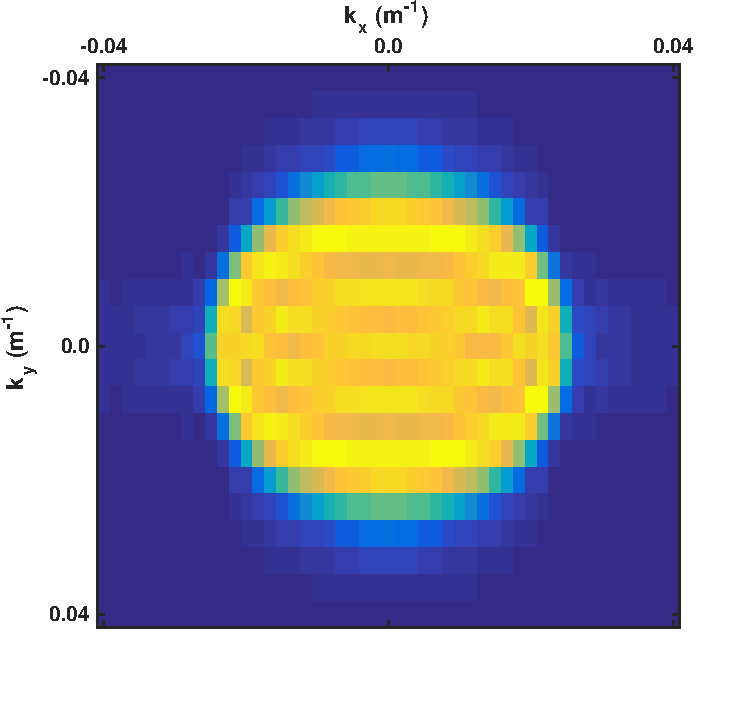
\includegraphics[width=\textwidth]{Plots/IdealData3d/P_f_slice40}
		\caption{}
		\label{fig:Ch-Theory-FK-f_slice-data}
	\end{subfigure}
	%
	\centering
	\begin{subfigure}[t]{0.3\textwidth}
		\centering
		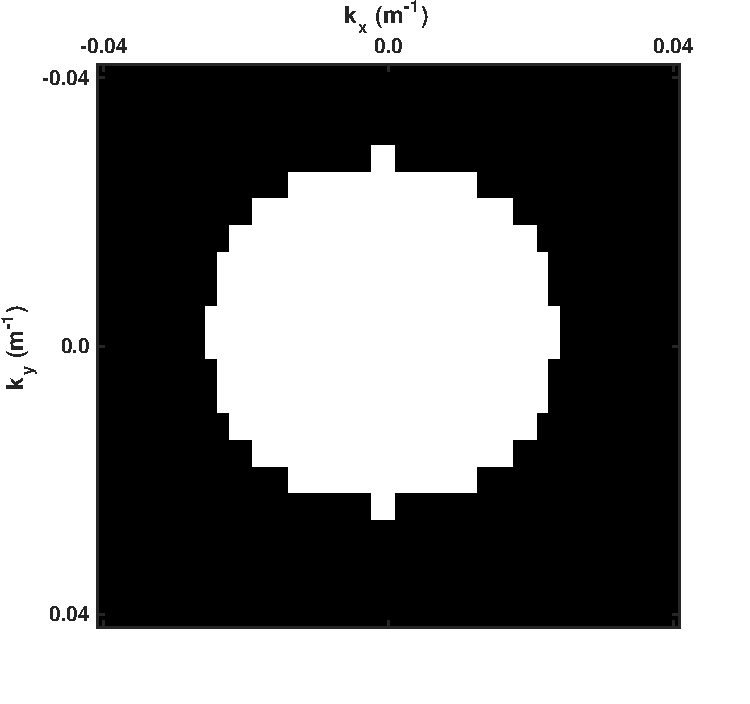
\includegraphics[width=\textwidth]{Plots/IdealData3d/fkk-mask-slice40}
		\caption{}
		\label{fig:Ch-Theory-FK-f_slice-mask}
	\end{subfigure}
	%
	\centering
	\begin{subfigure}[t]{0.3\textwidth}
		\centering
		\includegraphics[width=\textwidth]{Plots/IdealData3d/fk-slices/3dfk-cone}
		\caption{}
		\label{fig:Ch-Theory-FK-f_slice-data3d}
	\end{subfigure}
	
	\begin{subfigure}[t]{\textwidth}
		\centering
		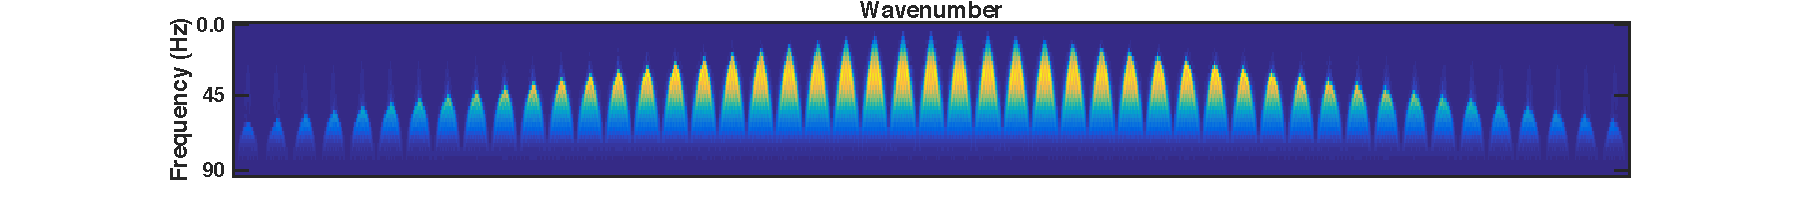
\includegraphics[width=0.9\textwidth]{Plots/IdealData3d/P_fkk_Delphi}
		\caption{}
		\label{fig:Ch-Theory-FK-delphi-data}
	\end{subfigure}
	\par\bigskip
	\begin{subfigure}[t]{\textwidth}
		\centering
		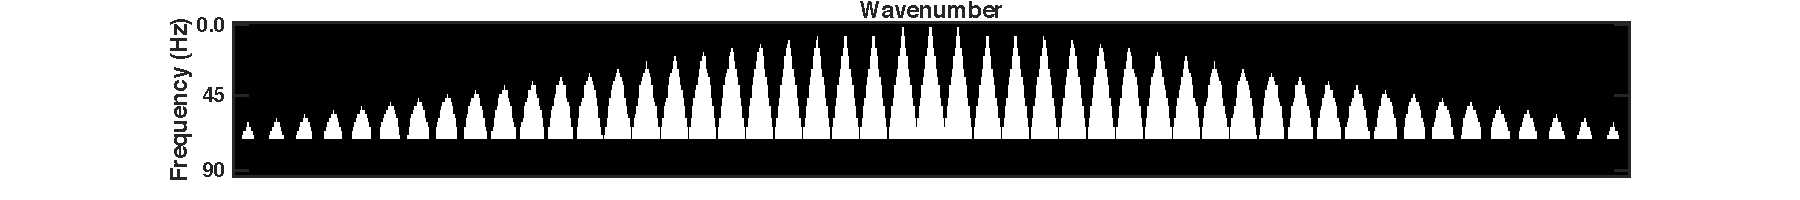
\includegraphics[width=0.9\textwidth]{Plots/IdealData3d/fkk-mask-Delphi}
		\caption{}
		\label{fig:Ch-Theory-FK-delphi-mask}
	\end{subfigure}
	
	\caption{Illustration of the 3D $f$-$k_x$-$k_y$ filter. (a) is a \SI{40}{\hertz} frequency slice of the $f$-$k_x$-$k_y$ spectrum of the data in Figure \ref{fig:Ch-Theory-DataSorting}. $k_x$ and $k_y$ refer to the crossline and inline wavenumber respectively. (b) is a \SI{40}{\hertz} frequency slice of the $f$-$k_x$-$k_y$ mask, where the white area equals 1 and the black area is 0. (c) shows the \SI{40}{\hertz} frequency slice of (a) sorted in a 3D cube. The red cone represents the edge of the 3D $f$-$k_x$-$k_y$ filter mask. (d) and (e) display the $f$-$k_x$-$k_y$ data spectrum and mask sorted according to section \ref{sec:Ch-Theory-3dExtension-DataSorting}, i.e. each sub-cone refers to one inline wavenumber. Note that due to the sorting the wavenumber axis is a mix of crossline and inline wavenumbers. For this reason the wavenumber axis has no labels.}
	\label{fig:Ch-Theory-FKK-Mask}

\end{figure}



\begin{figure}

	\centering 
	\begin{subfigure}[t]{0.45\textwidth}
		\centering
		\includegraphics[width = 0.65\textwidth]{Plots/IdealData3d/fkk-mask-slice40-2d}
		\caption{}
		\label{fig:Ch-Mahdad3d-2dfk-slice}
	\end{subfigure}
	
	\par\bigskip
	
	\centering
	\begin{subfigure}[t]{\textwidth}
		\centering
		\includegraphics[width = 0.9\textwidth]{Plots/IdealData3d/fkk-mask-Delphi-2d}
		\caption{}
		\label{fig:Ch-Mahdad3d-2dfk-Delphi}
	\end{subfigure}
	
	\caption{2D $f$-$k_x$ filter for 3D data. (a) shows a \SI{40}{\hertz} frequency slice of the $f$-$k_x$-$k_y$ spectrum, where the white area equals 1 and the black area is 0. Note that the filter is not affecting the inline wavenumbers $k_y$. (b) illustrates the 2D $f$-$k_x$ filter sorted according to section \ref{sec:Ch-Theory-3dExtension-DataSorting}. Each cone represents a 2D $f$-$k$ filter for a single inline wavenumber.}
	\label{fig:Ch-Mahdad3d-2dfk}
\end{figure}



\begin{comment}
Once the mask is built for a 5D data array it can either be applied to filter a 5D data array, or the mask is sorted to 2D according to section \ref{sec:Ch-Theory-3dExtension-DataSorting}, and applied to the $f$-$k_x$-$k_y$-spectrum of the data matrix (see Figure \ref{fig:Ch-Theory-FK-delphi-data}, \ref{fig:Ch-Theory-FK-delphi-mask}).
\end{comment}




\section{Results}

The 3D $f$-$k_x$-$k_y$ filter removes incoherent energy in the crossline and inline direction. The blended crossline sources design suggested in this thesis blends shots within the same crossline. Hence, an underlying question is whether the 3D $f$-$k_x$-$k_y$ filter in Figure \ref{fig:Ch-Theory-FKK-Mask} compared to the 2D $f$-$k$ filter in Figure \ref{fig:Ch-Mahdad3d-2dfk} provides significant deblending enhancements.

For this purpose the 3D synthetic common-receiver gather is used which is shown in Figure \ref{fig:Ch-Mahdad3d-Unbl-Delphi_xline} and \ref{fig:Ch-Mahdad3d-Unbl-Delphi}. The data are blended with the following parameters: Within each crossline there are 21 sources, which are blended in 3 experiments. For each experiment 7 randomly selected sources are blended with random time delays, i.e. the blending pattern with mixed incoherency is applied. The maximum allowed firing-time delay is set to \SI{400}{\milli\second}. The 3D incoherency value of the used blending matrix, $\mathbf{\Gamma}$, is $\mu = \SI{80.7}{\percent}$. 

The blended data are deblended with the 3D deblending algorithm. In one case a 2D $f$-$k$ filter is applied (see Figure \ref{fig:Ch-Mahdad3d-Deblending-2dfk}). In the other case a 3D $f$-$k_x$-$k_y$ filter is applied (see Figure \ref{fig:Ch-Mahdad3d-Deblending-3dfk}). It is clearly visible that the deblending quality increases significantly with the 3D $f$-$k_x$-$k_y$ filter. Figure \ref{fig:Ch-Mahdad3d-Deblending-2dvs3d-fk-tslice} displays a $\SI{420}{\milli\second}$ time slice of each subplot in Figure \ref{fig:Ch-Mahdad3d-Deblending-2dvs3d-fk}.

\begin{figure}
	
	\centering
	\begin{subfigure}[t]{0.2\textwidth}
		\centering
		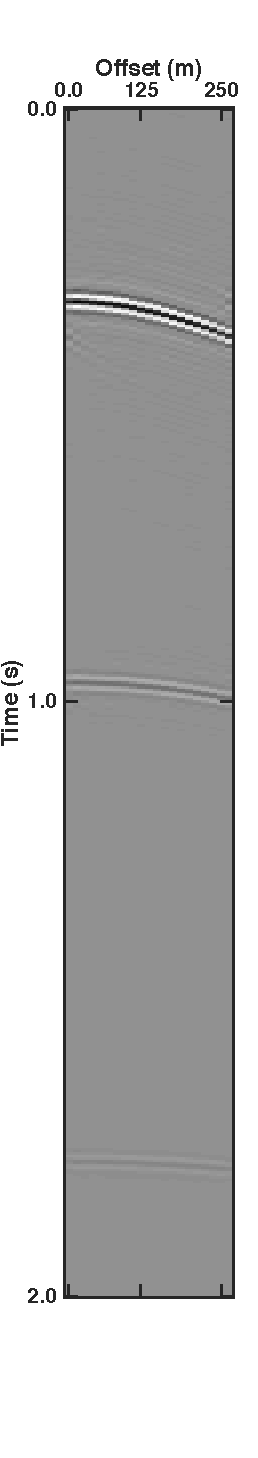
\includegraphics[width = \textwidth]{Plots/2dvs3dfk/xline_slices/Unblended_xline10}
		\caption{}
		\label{fig:Ch-Mahdad3d-Unbl-Delphi_xline}
	\end{subfigure}
	%
	\centering
	\begin{subfigure}[t]{0.2\textwidth}
		\includegraphics[width = \textwidth]{Plots/2dvs3dfk/xline_slices/Pseudo_xline10}
		\caption{}
		\label{fig:Ch-Mahdad3d-Deblending-Pseudo-xline}
	\end{subfigure}
	%
	\centering
	\begin{subfigure}[t]{0.2\textwidth}
		\includegraphics[width = \textwidth]{Plots/2dvs3dfk/xline_slices/Deblended_xline10_2d}
		\caption{}
		\label{fig:Ch-Mahdad3d-Deblending-2dfk_xline}
	\end{subfigure}
	%
	\centering
	\begin{subfigure}[t]{0.2\textwidth}
		\includegraphics[width = \textwidth]{Plots/2dvs3dfk/xline_slices/Deblended_xline10}
		\caption{}
		\label{fig:Ch-Mahdad3d-Deblending-3dfk_xline}
	\end{subfigure}
	
	\caption{(a) shows a crossline slice of a 3D synthetic common-receiver gather. The data are acquired with a source grid of 21 crossline shots and 51 inline shots. The data are blended with a mixed incoherency blending pattern. Then, the 3D deblending algorithm is applied. (b) shows the pseudo-deblended data. In case (c) the deblending algorithm uses a 2D $f$-$k_x$ filter. In case (d) it uses a 3D $f$-$k_x$-$k_y$ filter.}
	\label{fig:Ch-Mahdad3d-Deblending-2dvs3d-fk_xline}
	
\end{figure}

 
\begin{figure}
	
	\centering
	\begin{subfigure}[t]{0.8\textwidth}
		\centering
		\includegraphics[width = \textwidth]{Plots/BlendingPatterns/Unblended_Delphi_zoom-font14}
		\caption{Unblended synthetic data}
		\label{fig:Ch-Mahdad3d-Unbl-Delphi}
	\end{subfigure}

	\par\bigskip
	
	\centering
	\begin{subfigure}[t]{0.8\textwidth}
		\includegraphics[width = \textwidth]{Plots/BlendingPatterns/Pseudo-Deblendedv5_xt_100}
		\caption{Pseudo-deblended data}
		\label{fig:Ch-Mahdad3d-Deblending-Pseudo-Zoom}
	\end{subfigure}
	
	\par\bigskip

	\centering
	\begin{subfigure}[t]{0.8\textwidth}
		\includegraphics[width = \textwidth]{Plots/2dvs3dfk/Deblendedv6_xt_100}
		\caption{Deblended data with a 2D $f$-$k_x$ filter}
		\label{fig:Ch-Mahdad3d-Deblending-2dfk}
	\end{subfigure}
	
	\par\bigskip
	
	\centering
	\begin{subfigure}[t]{0.8\textwidth}
		\includegraphics[width = \textwidth]{Plots/2dvs3dfk/Deblendedv5_xt_100}
		\caption{Deblended data with a 3D $f$-$k_x$-$k_y$ filter}
		\label{fig:Ch-Mahdad3d-Deblending-3dfk}
	\end{subfigure}
	
	\caption{Illustration of the data in Figure \ref{fig:Ch-Mahdad3d-Deblending-2dvs3d-fk_xline} in 2D-view. The shown sections zoom on the strongest events. (a) shows the unblended data, and (b) the pseudo-deblended data. The deblended data in (c) is achieved with a deblending algorithm which uses a 2D $f$-$k_x$ filter. The deblended data in (d) is achieved with a deblending algorithm which uses a 3D $f$-$k_x$-$k_y$ filter.}
	\label{fig:Ch-Mahdad3d-Deblending-2dvs3d-fk}
	
\end{figure}


\begin{figure}
	
	\centering
	\begin{subfigure}[t]{0.45\textwidth}
		\centering
		\includegraphics[width = \textwidth]{Plots/BlendingPatterns/time-slices/Unblendedv5_100-tslice}
		\caption{Unblended synthetic data}
		\label{fig:Ch-Mahdad3d-Unbl-Delphi-tslice}
	\end{subfigure}
	%
	\centering
	\begin{subfigure}[t]{0.45\textwidth}
		\includegraphics[width = \textwidth]{Plots/BlendingPatterns/time-slices/Pseudo-Deblendedv5_xt_100-tslice_b7}
		\caption{Pseudo-deblended data}
		\label{fig:Ch-Mahdad3d-Deblending-Pseudo-Zoom-tslice}
	\end{subfigure}
	
	\par\bigskip

	\centering
	\begin{subfigure}[t]{0.45\textwidth}
		\includegraphics[width = \textwidth]{Plots/BlendingPatterns/time-slices/Deblendedv6_xt_100-tslice}
		\caption{Deblended data with a 2D $f$-$k_x$ filter}
		\label{fig:Ch-Mahdad3d-Deblending-2dfk-tslice}
	\end{subfigure}
	%
	\centering
	\begin{subfigure}[t]{0.45\textwidth}
		\includegraphics[width = \textwidth]{Plots/BlendingPatterns/time-slices/Deblendedv5_xt_100-tslice}
		\caption{Deblended data with a 3D $f$-$k_x$-$k_y$ filter}
		\label{fig:Ch-Mahdad3d-Deblending-3dfk-tslice}
	\end{subfigure}
	
	\caption{(a) - (d) show \SI{420}{\milli\second} time slices of the data in Figure \ref{fig:Ch-Mahdad3d-Deblending-2dvs3d-fk}.}
	\label{fig:Ch-Mahdad3d-Deblending-2dvs3d-fk-tslice}
	
\end{figure}


The deblending performance achieved with 2D and 3D filters is compared as a function of the maximum firing-time delay. For this purpose the data shown in Figure \ref{fig:Ch-Mahdad3d-Unbl-Delphi_xline} and \ref{fig:Ch-Mahdad3d-Unbl-Delphi} are blended with maximum firing-time delays varying between \SI{40}{\milli\second} and \SI{400}{\milli\second}. The blended data are deblended in one case with a 2D $f$-$k$ filter, and in the other case with a 3D $f$-$k_x$-$k_y$ filter. The resulting quality factors are shown in Figure \ref{fig:Ch-Mahdad3d-2dvs3dfk}. With a 3D $f$-$k_x$-$k_y$ filter a significantly higher deblending quality is achieved. Note that the quality difference between the 2D and 3D filter increases with increasing maximum firing-time delay. 
% Explanation: A larger maximum firing-time delay allows more blending noise energy to be built up in the inline direction. This energy is overseen by the 2D filter. Hence with increasing tg there is a increasing chance of passing noise.



\begin{figure}
	\centering
	\includegraphics[width = 0.6\textwidth]{Plots/2dvs3dfk/Q_2d-vs-3d_fk_v2}
	\caption{Comparison of the deblending quality with a 2D $f$-$k_x$ filter and a 3D $f$-$k_x$-$k_y$ filter. The data in Figure \ref{fig:Ch-Mahdad3d-Unbl-Delphi_xline} and \ref{fig:Ch-Mahdad3d-Unbl-Delphi} are blended with varying maximum firing-time delay. Then the blended data are deblended using a 2D $f$-$k_x$ filter and a 3D $f$-$k_x$-$k_y$ filter.}
	\label{fig:Ch-Mahdad3d-2dvs3dfk}
\end{figure}

\FloatBarrier


\section{Conclusions}

In this chapter I derived a 3D deblending method, which uses a coherency constraint. I demonstrated that 3D deblending significantly improves when the coherency constraint is extended to the crossline direction. Besides, I extended the incoherency measure, which I introduced in chapter \ref{chap:Incoherency}, from 2D to 3D. The synthetic data example showed that the difference in deblending quality of the 2D and 3D method increases with increasing maximum firing-time delay.  

Due to these observations I will deblend the complex synthetic data example in chapter \ref{chap:ComplexSynthetic} with a 3D deblending method, and I will use a 3D coherency constraint.



















